%% Basierend auf einer TeXnicCenter-Vorlage von Mark Müller
%%%%%%%%%%%%%%%%%%%%%%%%%%%%%%%%%%%%%%%%%%%%%%%%%%%%%%%%%%%%%%%%%%%%%%%

% Wählen Sie die Optionen aus, indem Sie % vor der Option entfernen  
% Dokumentation des KOMA-Script-Packets: scrguide

%%%%%%%%%%%%%%%%%%%%%%%%%%%%%%%%%%%%%%%%%%%%%%%%%%%%%%%%%%%%%%%%%%%%%%%
%% Optionen zum Layout des Artikels                                  %%
%%%%%%%%%%%%%%%%%%%%%%%%%%%%%%%%%%%%%%%%%%%%%%%%%%%%%%%%%%%%%%%%%%%%%%%
\documentclass[%
%a5paper,							% alle weiteren Papierformat einstellbar
%landscape,						% Querformat
%10pt,								% Schriftgröße (12pt, 11pt (Standard))
%BCOR1cm,							% Bindekorrektur, bspw. 1 cm
%DIVcalc,							% führt die Satzspiegelberechnung neu aus
%											  s. scrguide 2.4
%twoside,							% Doppelseiten
%twocolumn,						% zweispaltiger Satz
%halfparskip*,				% Absatzformatierung s. scrguide 3.1
%headsepline,					% Trennline zum Seitenkopf	
%footsepline,					% Trennline zum Seitenfuß
%titlepage,						% Titelei auf eigener Seite
%normalheadings,			% Überschriften etwas kleiner (smallheadings)
%idxtotoc,						% Index im Inhaltsverzeichnis
%liststotoc,					% Abb.- und Tab.verzeichnis im Inhalt
%bibtotoc,						% Literaturverzeichnis im Inhalt
%abstracton,					% Überschrift über der Zusammenfassung an	
%leqno,   						% Nummerierung von Gleichungen links
%fleqn,								% Ausgabe von Gleichungen linksbündig
%draft								% überlangen Zeilen in Ausgabe gekennzeichnet
]
{scrartcl}

%\pagestyle{empty}		% keine Kopf und Fußzeile (k. Seitenzahl)
%\pagestyle{headings}	% lebender Kolumnentitel

%% Deutsche Anpassungen %%%%%%%%%%%%%%%%%%%%%%%%%%%%%%%%%%%%%
\usepackage[english]{babel}
\usepackage[T1]{fontenc}
\usepackage[utf8]{inputenc}

\usepackage{amsthm} % Theorem-Packet
\usepackage{amsmath}
\usepackage{amssymb}

\usepackage{stmaryrd} % Blitzsymbol
\usepackage{fancyhdr} % Für Kopfzeile
\usepackage{graphicx} % Einbinden von Grafiken
\usepackage{bbding} % Für das Häckchen
\usepackage{amscd} % Kommutative Diagramme
\usepackage{mathtools} % Für das Definitionssymbol

\usepackage{listings}
\usepackage{courier}

\pagestyle{fancy}
\lhead{Computational Science I}\chead{Exercise notes: Real numbers}\rhead{HS 2013} % Kopfzeile

\newtheoremstyle{plain}%  name
  {.5\baselineskip}% Space above
  {.5\baselineskip}% Space below
  {}% Body font
  {}% Indent amount (empty = no indent, \parindent = para indent)
  {\bfseries}% Thm head font
  {:}% Punctuation after thm head
  { }% Space after thm head: " " = normal interword space; \newline = linebreak
  {}% Thm head spec (can be left empty, meaning `normal')
  
\makeatletter % Matrizen mit opitonalen Linien
\renewcommand*\env@matrix[1][*\c@MaxMatrixCols c]{%
  \hskip -\arraycolsep
  \let\@ifnextchar\new@ifnextchar
  \array{#1}}
\makeatother

\theoremstyle{plain}
\newtheorem*{bsp}{Beispiel} % Beispiele ohne Nummerierung
\newtheorem*{bws}{Beweis} % Beweise ohne Nummerierung 
\newenvironment{beweis}{\begin{bws}~\vspace{0.5\baselineskip}}{\hfill $\qedsymbol$\end{bws}}
\newenvironment{beispiel}{\begin{bsp}~\vspace{0.5\baselineskip}}{\end{bsp}}

\usepackage{lmodern} % Type1-Schriftart für nicht-englische Texte

\usepackage{enumerate}

\renewcommand\theenumi{\roman{enumi}}
\renewcommand\labelenumi{\theenumi)}

%% Packages für Grafiken & Abbildungen %%%%%%%%%%%%%%%%%%%%%%
%\usepackage{graphicx} %%Zum Laden von Grafiken
%\usepackage{subfig} %%Teilabbildungen in einer Abbildung
%\usepackage{tikz} %%Vektorgrafiken aus LaTeX heraus erstellen

%\setlength{\parindent}{0pt} % kein Einzug


%% Beachten Sie:
%% Die Einbindung einer Grafik erfolgt mit \includegraphics{Dateiname}
%% bzw. über den Dialog im Einfügen-Menü.
%% 
%% Im Modus "LaTeX => PDF" können Sie u.a. folgende Grafikformate verwenden:
%%   .jpg  .png  .pdf  .mps
%% 
%% In den Modi "LaTeX => DVI", "LaTeX => PS" und "LaTeX => PS => PDF"
%% können Sie u.a. folgende Grafikformate verwenden:
%%   .eps  .ps  .bmp  .pict  .pntg


%% Bibliographiestil %%%%%%%%%%%%%%%%%%%%%%%%%%%%%%%%%%%%%%%%%%%%%%%%%%
%\usepackage{natbib}

\begin{document}

\lstset{basicstyle=\ttfamily, breakatwhitespace=false, breaklines=true, frame=single, xleftmargin=\parindent, aboveskip=\baselineskip, belowskip=\baselineskip}

%\pagestyle{empty} %%Keine Kopf-/Fusszeilen auf den ersten Seiten.


%%%%%%%%%%%%%%%%%%%%%%%%%%%%%%%%%%%%%%%%%%%%%%%%%%%%%%%%%%%%%%%%%%%%%%%
%% Ihr Artikel                                                       %%
%%%%%%%%%%%%%%%%%%%%%%%%%%%%%%%%%%%%%%%%%%%%%%%%%%%%%%%%%%%%%%%%%%%%%%%

%% eigene Titelseitengestaltung %%%%%%%%%%%%%%%%%%%%%%%%%%%%%%%%%%%%%%%    
%\begin{titlepage}
%Einsetzen der TXC Vorlage "Deckblatt" möglich
%\end{titlepage}

%% Angaben zur Standardformatierung des Titels %%%%%%%%%%%%%%%%%%%%%%%%
\titlehead{\center{University of Zurich - HS 2013}}
%\subject{Typisierung}
\title{Computational Science I\\Exercise 1: Real numbers\\\rule{1.0\textwidth}{1.0pt}}
\author{Tobias Grubenmann}
%\and{Der Name des Co-Autoren}
%\thanks{Fußnote}			% entspr. \footnote im Fließtext
%\date{}							% falls anderes, als das aktuelle gewünscht
%\publishers{Herausgeber}

%% Widmungsseite %%%%%%%%%%%%%%%%%%%%%%%%%%%%%%%%%%%%%%%%%%%%%%%%%%%%%%
%\dedication{Widmung}

\maketitle 						% Titelei wird erzeugt

%% Zusammenfassung nach Titel, vor Inhaltsverzeichnis %%%%%%%%%%%%%%%%%
%\begin{abstract}
% Für eine kurze Zusammenfassung des folgenden Artikels.
% Für die Überschrift s. \documentclass[abstracton].
%\end{abstract}

%% Erzeugung von Verzeichnissen %%%%%%%%%%%%%%%%%%%%%%%%%%%%%%%%%%%%%%%
%\tableofcontents			% Inhaltsverzeichnis
%\listoftables				% Tabellenverzeichnis
%\listoffigures				% Abbildungsverzeichnis


%% Der Text %%%%%%%%%%%%%%%%%%%%%%%%%%%%%%%%%%%%%%%%%%%%%%%%%%%%%%%%%%%

\section*{Exercise 1}

Assuming Python uses \emph{unsigned} 32-bit integers to expressing time then the largest number for expressing time is \texttt{0xffffffff=4294967295}. We can use the Python interpreter to evaluate the highest time expression:

\lstinputlisting[language=Python]{../exercise01.py}

This evaluates to \lstinline{Sun Feb 07 07:28:15 2106}.

If Python uses \emph{signed} 32-bit integers to expressing time then teh largest number would be \texttt{0x7fffffff=2147483647} which evaluates to \lstinline{Tue Jan 19 04:14:07 2038}.

\section*{Exercise 2}

Assuming the floating point precision in Python follows the IEEE 754 standard, i.e. the mantissa is normalized and the highest and lowest exponent are treated different.

To get the bits of the mantissa we need to evaluate the smallest number $\varepsilon$ such that $1+\varepsilon>1$

To get the bits of the exponent we need to evaluate the greatest and smallest possible exponent to calculate the range of the exponent. The range is the difference of the greatest and the smallest exponent plus 1 for the zero. To get the greatest possible exponent we need to increase the exponent until we get an \emph{overflow exception} (plus 1 for the special treatment of the highest exponent). To get the smallest possible exponent we need to decrease the exponent until we get a loss of precision (plus 1 for the special treatment of the lowest exponent). The logarithm to the base 2 of the range gives us the number of bits for the exponent.

\lstinputlisting[language=Python]{../exercise02.py}

The outcome of the code above is 52 bits for the mantissa (+1 for the sign) and 11 bits for the exponent.

\section*{Exercise 3}

To use the Newton-Raphson method to find the $n$-th root of a number $x$ we define the following function $f$:
\begin{equation*}
f(y)=y^{n}-x
\end{equation*}
which has the derivative $f'(y)=n\cdot y^{n-1}$.

The function $f$ vanishes at the same points as the function $g(y)=y-\sqrt[n]{x}$ but doesn't need the root function (which we want to implement).

I implemented also a function to calculate $x^{n}$ since with the built-in \texttt{pow()} function we could directly calculate the $n$-th root and therefore my own function for the $n$-th root would be pointless.

The loop with the Newton-Raphson iteration stops when the absolute value of $\Delta x_{n+1}=\frac{f(x_{n})}{f'(x_{n})}$ is smaller than $x_{n}\cdot\varepsilon$ where $\varepsilon$ is the smallest number s.t. $1+\varepsilon>1$.

\lstinputlisting[language=Python]{../exercise03.py}

\section*{Exercise 4}

The code below generates the curlicues for $\mu\approx 2.24248$, $L=10000$ and $\mu\approx 4.12403$, $L=4459$:

\lstinputlisting[language=Python]{../exercise04.py}

\begin{center}
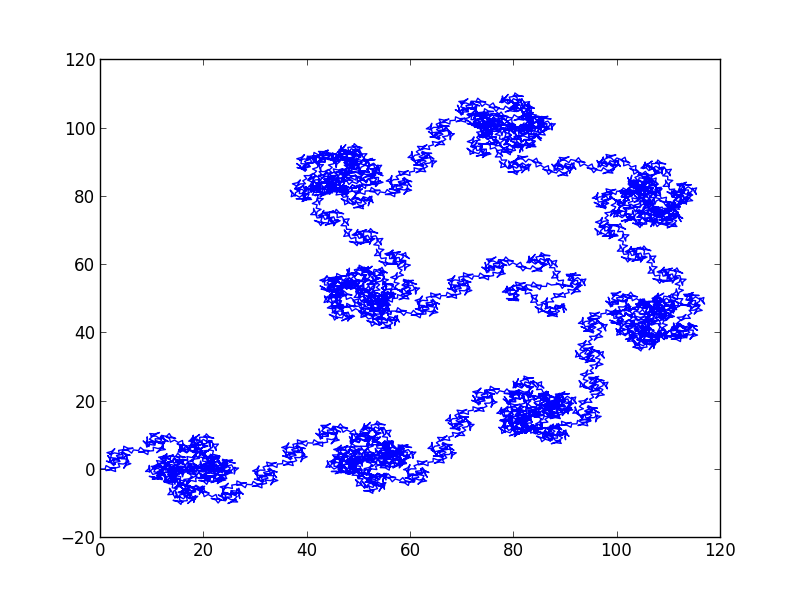
\includegraphics[width=0.6\linewidth]{../curlicue01.png}
\captionof{figure}{$\mu\approx 2.24248$, $L=10000$}
\end{center}

\begin{center}
\centering
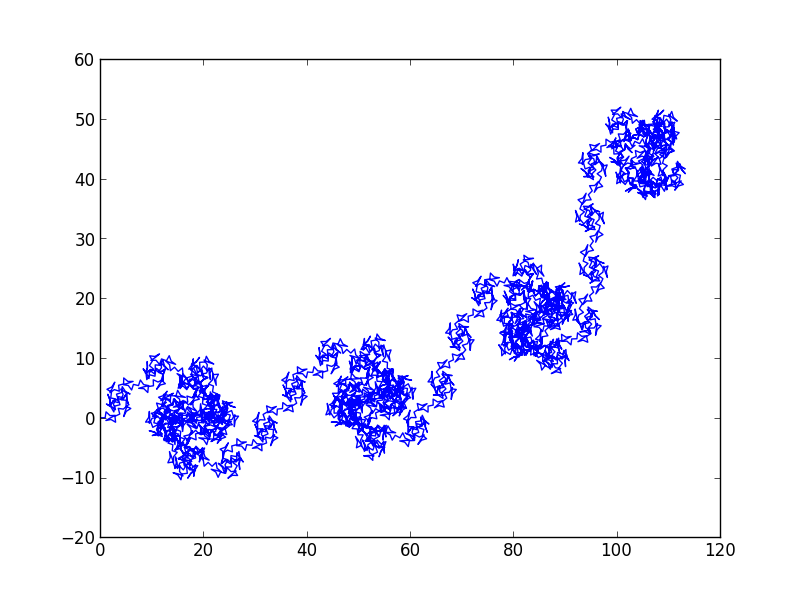
\includegraphics[width=0.6\linewidth]{../curlicue02.png}
\captionof{figure}{$\mu\approx 4.12403$, $L=4459$}
\end{center}

\section*{Exercise 5}

\texttt{pi(n)} returns $\pi$ up to $n$ digits. To get enough accuracy the first $n$ terms of the taylor series for the $arctan$ are evaluated. The approximation of $\pi$ is returned as a string.

\lstinputlisting[language=Python]{../exercise05.py}

The output for \texttt{pi(1000)} is:

\lstinputlisting{../output_exercise05.py}

%% Bibliographie unter Verwendung von dinnat %%%%%%%%%%%%%%%%%%%%%%%%%%
%\setbibpreamble{Präambel}		% Text vor dem Verzeichnis
%\bibliographystyle{dinat}
%\bibliography{bibliographie}	% Sie benötigen einen *.bib-Datei

\end{document}


